\documentclass[12pt]{report}
\usepackage[a4paper,margin=1in]{geometry}
\usepackage{setspace}
\usepackage{graphicx}
\usepackage{sectsty}
\usepackage{pdfpages}
% \usepackage{booktabs}
\usepackage[export]{adjustbox}
\usepackage{amssymb}
\usepackage{cancel}
\usepackage[numbered]{matlab-prettifier}
\usepackage{circuitikz}
\usepackage{xfrac}
\usepackage{lmodern}
\usepackage{multicol}
\usepackage{caption}
\usepackage{amsmath}
\usepackage{enumitem}
\usepackage{subcaption}

\newcommand{\eqname}[1]{\tag*{#1}}% Tag equation with name

\usetikzlibrary{arrows}
\graphicspath{{images/}}
\usetikzlibrary{calc,patterns,angles,quotes}

\allsectionsfont{\centering}
\renewcommand\thesection{\arabic{section}}
\renewcommand{\thefootnote}{\arabic{footnote}}
\setcounter{tocdepth}{5}

\begin{document}

\input{titlepage}
\pagenumbering{roman}
{\tableofcontents\let\clearpage\relax\listoffigures}
\clearpage
\pagenumbering{arabic}
\newpage
\begin{flushleft}
% ---------------------------------------------------------------------------- %
\section{Conceptualize the Problem}
% ---------------------------------------------------------------------------- %

\begin{figure}[h]
  \begin{minipage}[c]{.4\textwidth}
  \usetikzlibrary{calc,patterns,angles,quotes}
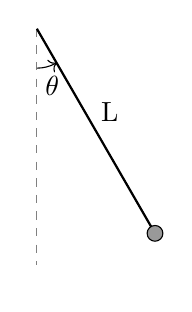
\begin{tikzpicture}
    % save length of g-vector and theta to macros
    \pgfmathsetmacro{\Gvec}{1.5}
    \pgfmathsetmacro{\myAngle}{30}
    % calculate lengths of vector components
    \pgfmathsetmacro{\Gcos}{\Gvec*cos(\myAngle)}
    \pgfmathsetmacro{\Gsin}{\Gvec*sin(\myAngle)}

    \coordinate (centro) at (0,0);
    \draw[dashed,gray,-] (centro) -- ++ (0,-3) node (mary) [black,below]{$ $};
    \draw[thick] (centro) -- ++(270+\myAngle:3) coordinate (bob);
    \pic [draw, ->, "$\theta$", angle eccentricity=1.5] {angle = mary--centro--bob};
    \draw (bob) -- (centro) node[midway, above]{~~~L};
    \filldraw [fill=black!40,draw=black] (bob) circle[radius=0.1];
\end{tikzpicture}

\end{minipage}%
\begin{minipage}[c]{.6\textwidth}
  The pendulumn system consists of two rigid bars rotating about one end,
  attached at the opposite ends by a linear spring.
\end{minipage}
\end{figure}

\subsection{Constants and Assumptions}
\begin{tabular}{ll@{\hskip .75in}l}
 \multicolumn{1}{c}{Constants:} && \multicolumn{1}{c}{Assumptions:} \\
 Bar Mass: &$m$ = 0.25kg & No Losses\\
 Bar Length: &$L$ = 0.5m & Released from Rest\\
 Gravity: &$g$ = 9.81$\sfrac{m}{s^2}$ &Slender Bars \\
 Linear Spring: &&Planar\\
 \quad Spring Coefficient:& $k = 25~\sfrac{N}{m}$ &Rigid-Body Dynamics \\
 \quad Unstretched Length:& $L$ \\
\end{tabular}
\vspace{5ex}

We are asked to determine the following: \\
\begin{enumerate}
  \item The 6 Equations / 6 Unknowns for the system to solve for the Equations of Motion.
  \item Integrate the Equations of Motion using various initial conditions.
  \begin{enumerate}
    \item $\theta_o = \sfrac{\pi}{12}~rad, \quad \phi_o = \sfrac{\pi}{12}~rad$
    \item $\theta_o = \sfrac{-\pi}{12}~rad, \quad \phi_o = \sfrac{\pi}{12}~rad$
    \item $\theta_o = \sfrac{\pi}{36}~rad, \quad \phi_o = \sfrac{\pi}{12}~rad$
  \end{enumerate}
  \item Linearize the Equations of Motion assuming small angular positions and velocities
  (i.e. small angle approximation $\sin(x) \approx x,~\cos(x) \approx 1$)
  \begin{itemize}
    \item Determine the A matrix below.
  \end{itemize}
\end{enumerate}
\begin{equation}
\begin{bmatrix}
  \ddot{\theta} \\
  \ddot{\phi}
\end{bmatrix}
=
\begin{bmatrix}
A
\end{bmatrix}
\begin{bmatrix}
\theta \\
\phi
\end{bmatrix}
\nonumber
\end{equation}
\begin{enumerate}[resume]
  \item Find the natural frequencies of the system and their respective eigenvectors
  using the eigenvalues and eigenvectors of [A].
  \item Using information from (5), solve for the analytical solution to the
  linearized Equations of Motion and plot them for the initial conditions defined in (2).
\end{enumerate}
\newpage

% ---------------------------------------------------------------------------- %
\section{Free Body Diagram}
% ---------------------------------------------------------------------------- %
\begin{figure}[ht]
   \begin{minipage}[c]{.225\textwidth}
      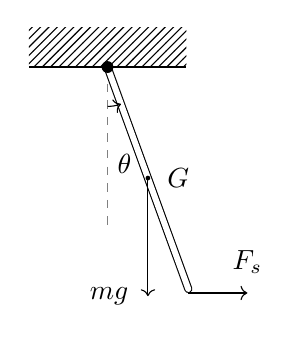
\begin{tikzpicture}

  \pgfmathsetmacro{\Gvec}{1.5}
  \pgfmathsetmacro{\myAngle}{20}

  \pgfmathsetmacro{\Gcos}{\Gvec*cos(\myAngle)}
  \pgfmathsetmacro{\Gsin}{\Gvec*sin(\myAngle)}

  \coordinate (centro) at (0,0);
  \draw[dashed,gray,-] (centro) -- ++ (0,-2) node (mary) [black,below]{$ $};
  \draw[double distance = .75mm,line cap=round] (centro) -- ++(270+\myAngle:3) coordinate (bob);
  \draw[->] (270+\myAngle:1.5) coordinate (g) -- ($(270+\myAngle:1.5) + (0,-1.5)$) coordinate (mg);
  \draw (mg) node[label=180:$mg$] {};
  \draw (g) node[label=east:$G$] {};
  \fill[black] (270+\myAngle:1.5) circle (0.03);
  \pic [draw,->, "$\theta$", angle eccentricity=2.5] {angle = mary--centro--bob};

  \fill[pattern = north east lines] ($ (centro) + (-1,0) $) rectangle ($ (centro) + (1,0.5) $);
  \draw[thick] ($ (centro) + (-1,0) $) -- ($ (centro) + (1,0) $);

  \fill[black] (centro) circle (0.075);

  (270+\myAngle:3) coordinate (bob2);

  \draw[->] ($ (bob) + (0,-.05) $) -- ++(0:.75) coordinate (fs);
  \draw (fs) node[label=north:$F_s$] {};

\end{tikzpicture}

   \end{minipage}%
   \begin{minipage}[c]{.55\textwidth}
     \center
     \begin{tabular}{rl}
     $F_s$:&Force onto bar by the spring\\
     $mg$:&Mass $\cdot$ gravity, weight of each bar\\
     $G$:&Center of gravity of each bar\\
     $\theta,~\phi$:& Angle of bar relative to vertical\\
     $A_n,~C_n$:& Reaction forces in the normal \\ & direction at pin\\
     $A_t,~C_t$:& Reaction forces in the tangential \\ & direction at pin\\
   \end{tabular}
   \end{minipage}%
  \begin{minipage}[c]{.225\textwidth}
    \vspace{2.8ex}
    \hspace{2ex}
     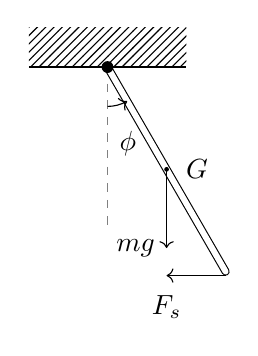
\begin{tikzpicture}

  \pgfmathsetmacro{\Gvec}{1.5}
  \pgfmathsetmacro{\myAngle}{30}

  \pgfmathsetmacro{\Gcos}{\Gvec*cos(\myAngle)}
  \pgfmathsetmacro{\Gsin}{\Gvec*sin(\myAngle)}

  \coordinate (centro) at (0,0);
  \draw[dashed,gray,-] (centro) -- ++ (0,-2) node (mary) [black,below]{$ $};
  \draw[double distance = .75mm,line cap=round] (centro) -- ++(270+\myAngle:3) coordinate (bob);
  \draw[->] (270+\myAngle:1.5) coordinate (g) -- ($(270+\myAngle:1.5) + (0,-1)$) coordinate (mg);
  \draw ($(mg) + (.1,0)$) node[label=180:$mg$] {};
  \draw (g) node[label=east:$G$] {};
  \fill[black] (270+\myAngle:1.5) circle (0.03);
  \pic [draw,->, "$\phi$", angle eccentricity=2] {angle = mary--centro--bob};

  \fill[pattern = north east lines] ($ (centro) + (-1,0) $) rectangle ($ (centro) + (1,0.5) $);
  \draw[thick] ($ (centro) + (-1,0) $) -- ($ (centro) + (1,0) $);

  \fill[black] (centro) circle (0.075);

  \draw[->] ($ (bob) + (0,-.05) $) -- ++(180:.75) coordinate (fs);
  \draw (fs) node[label=south:$F_s$] {};

\end{tikzpicture}

  \end{minipage}
\end{figure}
\vspace{-3ex}
\subsection*{Acceleration Diagram}
\begin{figure}[ht]
   \begin{minipage}[c]{.25\textwidth}
      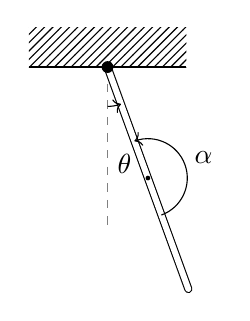
\begin{tikzpicture}

  \pgfmathsetmacro{\Gvec}{1.5}
  \pgfmathsetmacro{\myAngle}{20}

  \pgfmathsetmacro{\Gcos}{\Gvec*cos(\myAngle)}
  \pgfmathsetmacro{\Gsin}{\Gvec*sin(\myAngle)}

  \coordinate (centro) at (0,0);
  \draw[dashed,gray,-] (centro) -- ++ (0,-2) node (mary) [black,below]{$ $};
  \draw[double distance = .75mm,line cap=round] (centro) -- ++(270+\myAngle:3) coordinate (bob);
  % \draw[->] (270+\myAngle:1.5) coordinate (g) -- ($(270+\myAngle:1.5) + (0,-1.5)$) coordinate (mg);
  % \draw (mg) node[label=180:$mg$] {};
  \fill[black] (270+\myAngle:1.5) circle (0.03) coordinate (barcenter);
  \pic [draw,->, "$\theta$", angle eccentricity=2.5] {angle = mary--centro--bob};
  \pic [draw,->, "$\alpha$", angle eccentricity=1.5] {angle = bob--barcenter--centro};

  \fill[pattern = north east lines] ($ (centro) + (-1,0) $) rectangle ($ (centro) + (1,0.5) $);
  \draw[thick] ($ (centro) + (-1,0) $) -- ($ (centro) + (1,0) $);

  \fill[black] (centro) circle (0.075);

\end{tikzpicture}

   \end{minipage}%
   \begin{minipage}[c]{.5\textwidth}
     \center
     \begin{tabular}{rl}
     $\alpha$:& $\ddot{\theta},~\ddot{\phi}$ respectively\\
   \end{tabular}
   \end{minipage}%
  \begin{minipage}[c]{.25\textwidth}
    % \vspace{2.8ex}
    \hspace{2ex}
     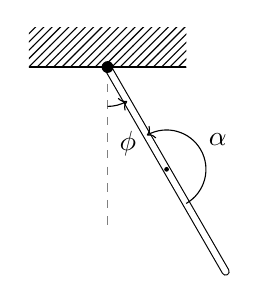
\begin{tikzpicture}

  \pgfmathsetmacro{\Gvec}{1.5}
  \pgfmathsetmacro{\myAngle}{30}

  \pgfmathsetmacro{\Gcos}{\Gvec*cos(\myAngle)}
  \pgfmathsetmacro{\Gsin}{\Gvec*sin(\myAngle)}

  \coordinate (centro) at (0,0);
  \draw[dashed,gray,-] (centro) -- ++ (0,-2) node (mary) [black,below]{$ $};
  \draw[double distance = .75mm,line cap=round] (centro) -- ++(270+\myAngle:3) coordinate (bob);
  % \draw[->] (270+\myAngle:1.5) coordinate (g) -- ($(270+\myAngle:1.5) + (0,-1)$) coordinate (mg);
  % \draw ($(mg) + (.1,0)$) node[label=180:$mg$] {};
  \fill[black] (270+\myAngle:1.5) circle (0.03) coordinate (bar2center);
  \pic [draw,->, "$\phi$", angle eccentricity=2] {angle = mary--centro--bob};
  \pic [draw,->, "$\alpha$", angle eccentricity=1.5] {angle = bob--bar2center--centro};

  \fill[pattern = north east lines] ($ (centro) + (-1,0) $) rectangle ($ (centro) + (1,0.5) $);
  \draw[thick] ($ (centro) + (-1,0) $) -- ($ (centro) + (1,0) $);

  \fill[black] (centro) circle (0.075);

\end{tikzpicture}

  \end{minipage}
\end{figure}
\vspace{-5ex}
% ---------------------------------------------------------------------------- %
\section{Coordinate Frame}
% ---------------------------------------------------------------------------- %
\begin{figure}[ht]
    \begin{subfigure}[t]{.5\textwidth}
      \center
      \caption{Separate Coordinate Frames}
      \label{coord:a}
      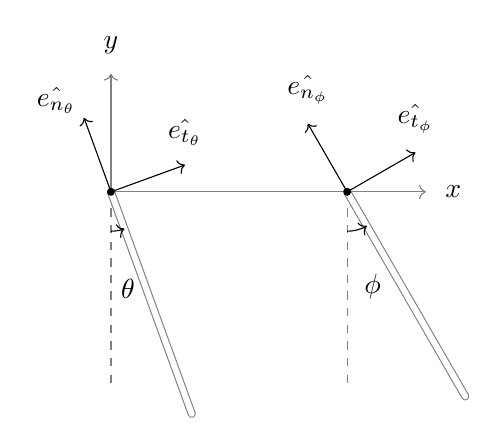
\begin{tikzpicture}

  \pgfmathsetmacro{\Gvec}{1.5}
  \pgfmathsetmacro{\myAngle}{20}

  \pgfmathsetmacro{\Gcos}{\Gvec*cos(\myAngle)}
  \pgfmathsetmacro{\Gsin}{\Gvec*sin(\myAngle)}

  \coordinate (centro) at (0,0);
  \draw[dashed,gray,-] (centro) -- ++ (0,-2.5) node (mary) [black,below] {};
  \draw[double distance = .75mm,line cap=round,gray] (centro) -- ++(270+\myAngle:3) coordinate (bob);

  \draw[->] (centro) -- ++(270+\myAngle:-1) coordinate (normL);
  \draw (normL) node[label={[label distance=-2mm]110:$\hat{e_{n_{\theta}}}$}] {};
  \draw[->] (centro) -- ++(20:1) coordinate (tanL);
  \draw (tanL) node[label=$\hat{e_{t_{\theta}}}$] {};
  \pic [draw,->, "${\theta}$", angle eccentricity=2.5] {angle = mary--centro--bob};



  \pgfmathsetmacro{\Gvec}{1.5}
  \pgfmathsetmacro{\myAngle}{30}

  \pgfmathsetmacro{\Gcos}{\Gvec*cos(\myAngle)}
  \pgfmathsetmacro{\Gsin}{\Gvec*sin(\myAngle)}

  \coordinate (centro) at (3,0);
  \draw[dashed,gray,-] (centro) -- ++ (0,-2.5) node (mary) [black,below] {};
  \draw[double distance = .75mm,line cap=round,gray] (centro) -- ++(270+\myAngle:3) coordinate (bob);

  \draw[->] (centro) -- ++(270+\myAngle:-1) coordinate (normR);
  \draw (normR) node[label=$\hat{e_{n_{\phi}}}$] {};
  \draw[->] (centro) -- ++(30:1) coordinate (tanR);
  \draw (tanR) node[label=$\hat{e_{t_{\phi}}}$] {};

  \pic [draw,->, "${\phi}$", angle eccentricity=2.5] {angle = mary--centro--bob};



  \draw [->,gray] (0,0) -- ++ (0:4) coordinate (x);
  \draw [->,gray] (0,0) -- ++ (90:1.5) coordinate (y);
  \draw (x) node[label=0:$x$] {};
  \draw (y) node[label=90:$y$] {};
  \fill[black] (centro) circle (0.05);
  \fill[black] (0,0) circle (0.05);
\end{tikzpicture}

      \vspace{2ex}
    \end{subfigure}%
\begin{subfigure}[t]{.5\textwidth}
      \center
      \caption{Unit Vector Calculations}
      \label{coord:b}
      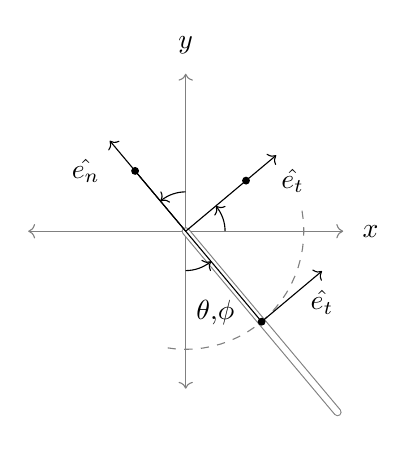
\begin{tikzpicture}

  \pgfmathsetmacro{\Gvec}{1.5}
  \pgfmathsetmacro{\myAngle}{40}

  \draw [->,gray] (0,0) -- ++ (0:2) coordinate (x);
  \draw [->,gray] (0,0) -- ++ (0:-2);
  \draw [->,gray] (0,0) -- ++ (90:2) coordinate (y);
  \draw [->,gray] (0,0) -- ++ (90:-2);
  \draw (x) node[label=0:$x$] {};
  \draw (y) node[label=90:$y$] {};

  \pgfmathsetmacro{\Gcos}{\Gvec*cos(\myAngle)}
  \pgfmathsetmacro{\Gsin}{\Gvec*sin(\myAngle)}

  \coordinate (centro) at (0,0);
  \coordinate (centro) -- ++ (0,-2.5) node (mary) {};
  \draw[double distance = .75mm,line cap=round,gray] (centro) -- ++(270+\myAngle:3) coordinate (bob);

  \draw[->] (centro) -- ++(270+\myAngle:-1.5) coordinate (norm);
  % \draw (norm) node[label=$\hat{e_n}$] {};
  \draw[->] (centro) -- ++(40:1.5) coordinate (tan);
  % \draw (tan) node[label=$\hat{e_t}$] {};
  \pic [draw,->, "$\theta\textrm{,}\phi$", angle eccentricity=2.2] {angle = mary--centro--bob};

  % \fill[black] (centro) circle (0.05);
  % \fill[black] (0,0) circle (0.05);


  \pic [draw,->, "$ $", angle eccentricity=2] {angle = x--centro--tan};
  \pic [draw,->, "$ $", angle eccentricity=2] {angle = y--centro--norm};

  \draw[gray,dashed,domain=10:-100] (centro) plot ({1.5*cos(\x)}, {1.5*sin(\x)});
  \fill[black] (centro) -- ++(40:1) circle (0.05) coordinate (co1);
  \draw (co1) node[label={[label distance=2mm]0:$\hat{e_t}$}] {};
  \fill[black] (centro) -- ++(130:1) circle (0.05) coordinate (co2);
  \draw (co2) node[label={[label distance=2mm]180:$\hat{e_n}$}] {};
  \fill[black] (270+\myAngle:1.5) circle (0.05);
  \draw[->] (270+\myAngle:1.5) -- ++(40:1) coordinate (tan2);
  \draw (270+\myAngle:1.5) -- (co2);
  \draw (tan2) node[label=-90:$\hat{e_t}$] {};

\end{tikzpicture}
 \\
      \begin{tabular}{rl}
        $\hat{e_n}:$ & $\left[\textrm{-}\sin(\theta)\hat{\textrm{\i}}+\cos(\theta)\hat{\textrm{\j}}\right]$ \\
        $\hat{e_t}:$ & $\left[\cos(\theta)\hat{\textrm{\i}}+\sin(\theta)\hat{\textrm{\j}}\right]$ \\
      \end{tabular}
    \end{subfigure}
    \caption{Visual Representation of Coordinate Frame Unit Vectors}
\end{figure}
Due to the complexity of the sytem if it were to be defined in cartesian coordinates,
we determined that the motion of the system would most effectively be represented by two separate
normal-tangential coordinate frames because the motion of each bar is purely rotational, where the
center of mass of each bar is following a curve. As seen in Figure (\ref{coord:a}), two coordinate
frames were used, one for each bar. Similarly, Figure (\ref{coord:b}) shows how the
unit vectors are calculated as well as the path the center of mass travels.
\newpage

% ---------------------------------------------------------------------------- %
\section{Sum of Forces}
% ---------------------------------------------------------------------------- %
The six equations that represent the forces on the system are comprised of four force summations and two moment equations,
\begin{align}
  \sum F_n &= m\frac{L}{2}\dot{\theta}^2 = F_{s_n} + A_n - mg\cos(\theta) \label{force_left_bar_theta_normal} \\ \eqname{Sum of Normal Forces on the left bar ($\theta$)} \\
  \sum F_t &= m\frac{L}{2}\ddot{\theta} = F_{s_n} + A_t- mg\sin(\theta) \label{force_left_bar_theta_tangential} \\ \eqname{Sum of Tangential Forces on the left bar ($\theta$)} \\
  \sum F_n &= m\frac{L}{2}\dot{\phi}^2 = F_{s_n} + C_n - mg\cos(\phi) \label{force_right_bar_phi_normal} \\ \eqname{Sum of Normal Forces on the right bar ($\phi$)} \\
  \sum F_t &= m\frac{L}{2}\ddot{\phi} = F_{s_n} + C_t- mg\sin(\phi) \label{force_right_bar_phi_tangential} \\ \eqname{Sum of Tangential Forces on the right bar ($\phi$)} \\
% \end{align}
% \begin{align}
  \sum M_A &= -\left(\frac{L}{2} \cdot mg\sin(\theta)\right) + \left(F_{st} \cdot L\right) = \frac{1}{3}mL^2\ddot{\theta} \label{moment_left_bar_theta} \\ \eqname{Sum of Moments about A ($\theta$)} \\
  \sum M_C &= -\left(\frac{L}{2} \cdot mg\sin(\phi)\right)+\left(F_{st} \cdot L\right) = \frac{1}{3}mL^2\ddot{\phi} \label{moment_right_bar_theta} \\ \eqname{Sum of Moments about C ($\phi$)}
\end{align}
Where: \\
~\\
\begin{tabular}{rl}
$\theta$:& Position of the left bar. \\
$\phi$:& Position of the right bar. \\
$\dot{\theta}$:& Angular velocity of the left bar. \\
$\dot{\phi}$:& Angular velocity of the right bar. \\
$\ddot{\theta}$:& Angular acceleration of the left bar. \\
$\ddot{\phi}$:& Angular acceleration of the right bar. \\
$A$:& Reaction force in the normal or tangential direction on the left bar. \\
$C$:& Reaction force in the normal or tangential direction on the right bar. \\
$F_s$:& Force due to the spring in either the normal or tangential direction. \\
$m,~L,~g$: & Mass, length of each bar, and gravity, respectively.
\end{tabular}
% ---------------------------------------------------------------------------- %
\section{Knowns and Unknowns} \label{knownsandunknowns}
% ---------------------------------------------------------------------------- %
\begin{tabular}{ll@{\hskip .75in}ll}
  \multicolumn{1}{c}{Knowns:} && \multicolumn{1}{c}{Unknowns:} \\
  Mass: &$m$ = 0.25kg & Reaction Forces: & $A_n,~A_t$ \\
  String Length: &$L$ = 0.5m & & $C_n,~C_t$\\
  Gravity: &$g$ = 9.81$\sfrac{m}{s^2}$& Angular Accelerations: & $\ddot{\theta},~\ddot{\phi}$ \\
  Linear Spring: \\
  \quad Spring Coefficient:& $k = 25~\sfrac{N}{m}$\\
  \quad Unstretched Length:& $L$ \\
  State Variables: \\
  \quad Angular Position: &$\theta,~\phi$ & \\
  \quad Angular Velocity: &$\dot{\theta},~\dot{\phi}$ & \\
\end{tabular}
\vspace{2ex}

Since there are six equations and six unknowns, we can solve for the equations of
motion analytically using Matlab.

% ---------------------------------------------------------------------------- %
\section{Constraints}
% ---------------------------------------------------------------------------- %
No constraint equations were needed to find a solution to the system.
% ---------------------------------------------------------------------------- %
\section{Solve for the Equations of Motion}
% ---------------------------------------------------------------------------- %

% ---------------------------------------------------------------------------- %
\section{Solve the Equations of Motion}
% ---------------------------------------------------------------------------- %
\begin{figure}[ht]
  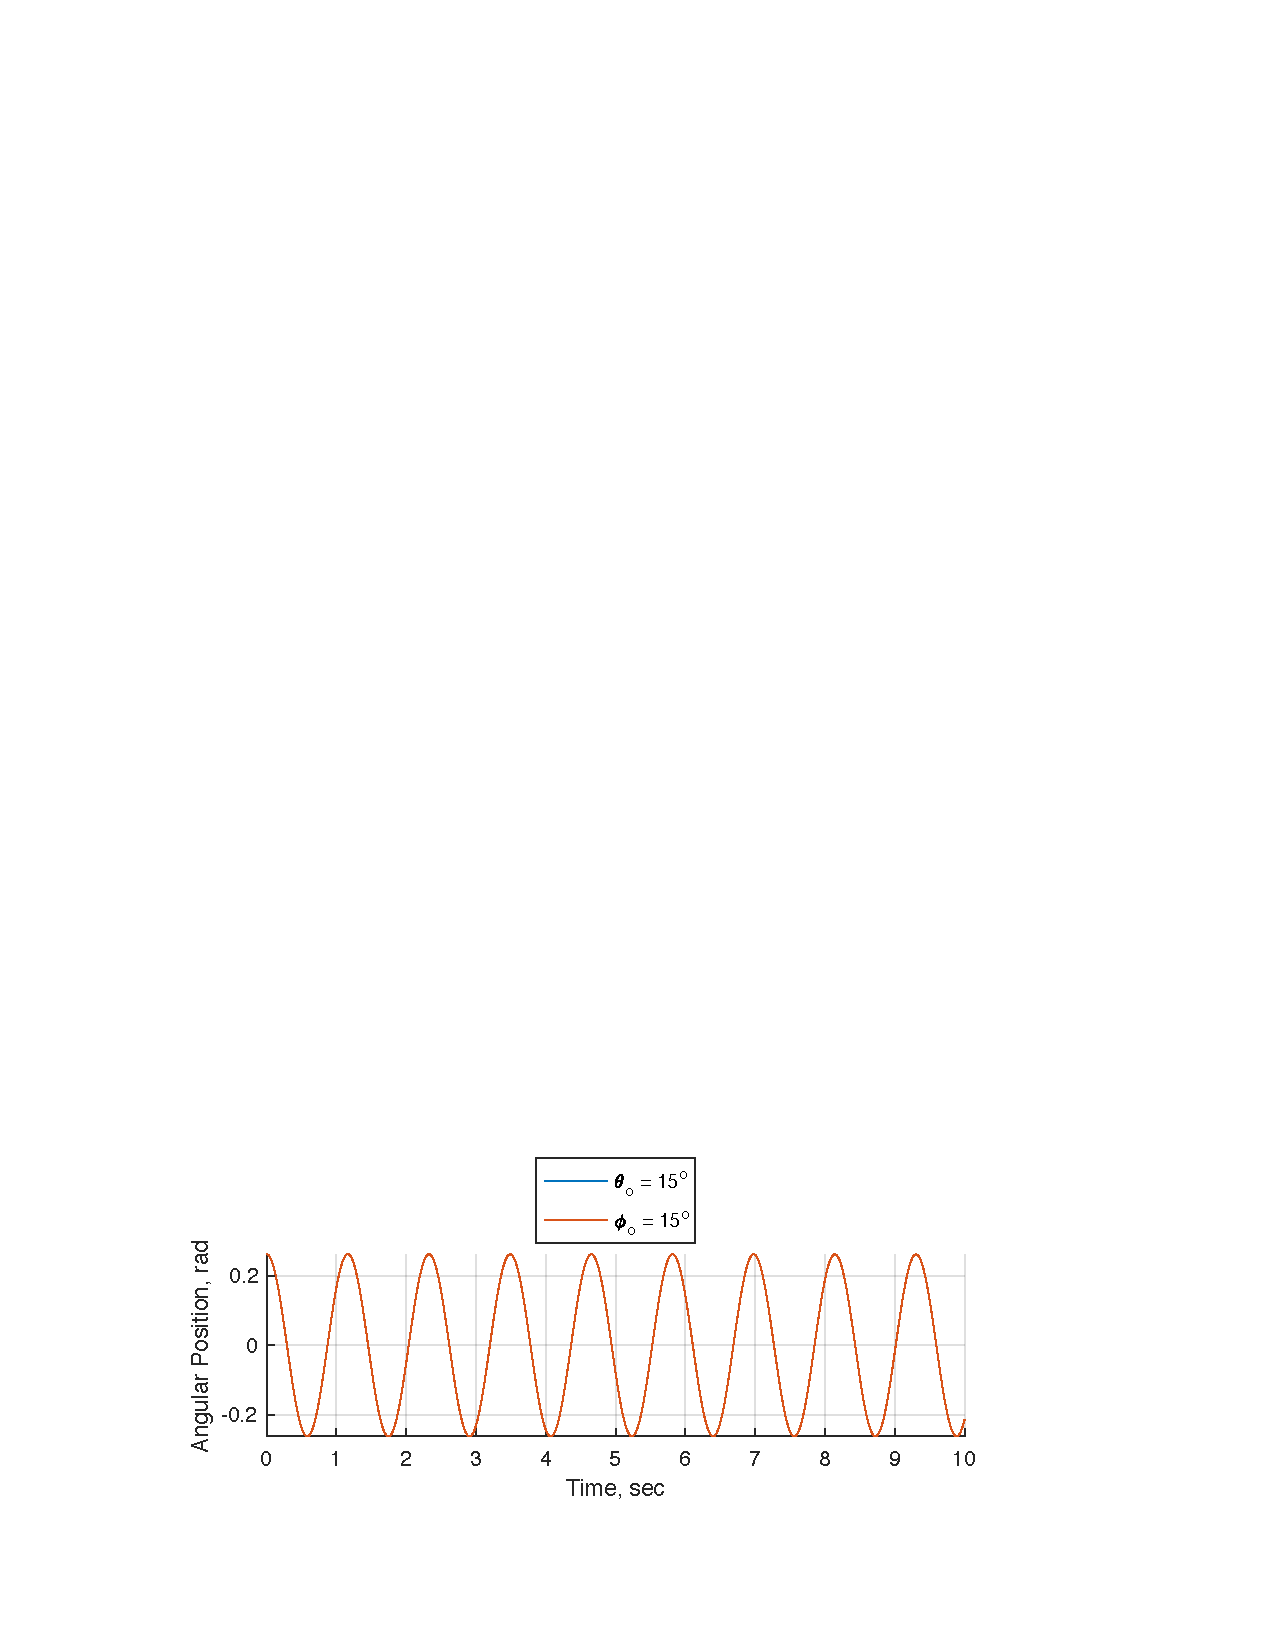
\includegraphics[center]{1}
  \caption{Angular Position vs. Time ($\theta_o:~15^\circ,~\phi_o:~15^\circ$)}
\end{figure}
\begin{figure}[ht]
  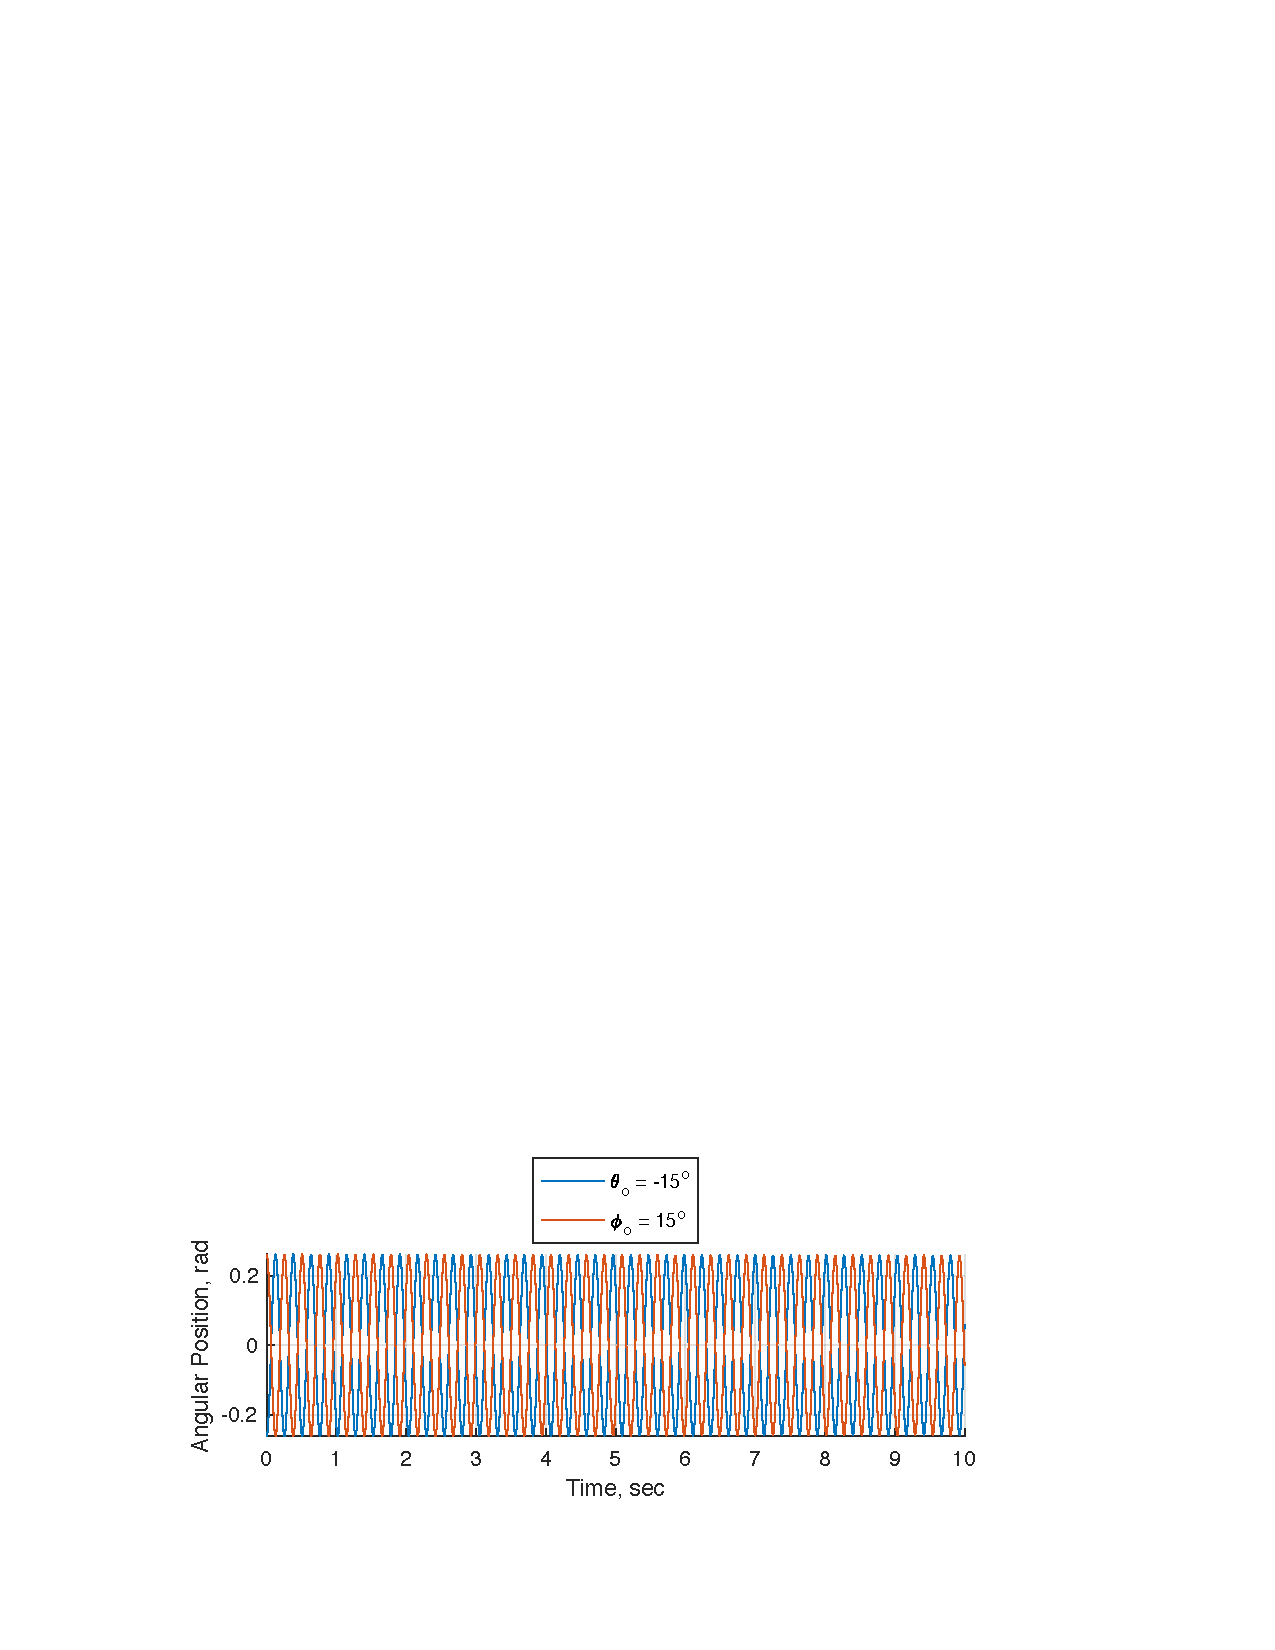
\includegraphics[center]{2}
  \caption{Angular Position vs. Time ($\theta_o:~\textrm{-}15^\circ,~\phi_o:~15^\circ$)}
\end{figure}
\begin{figure}[ht]
  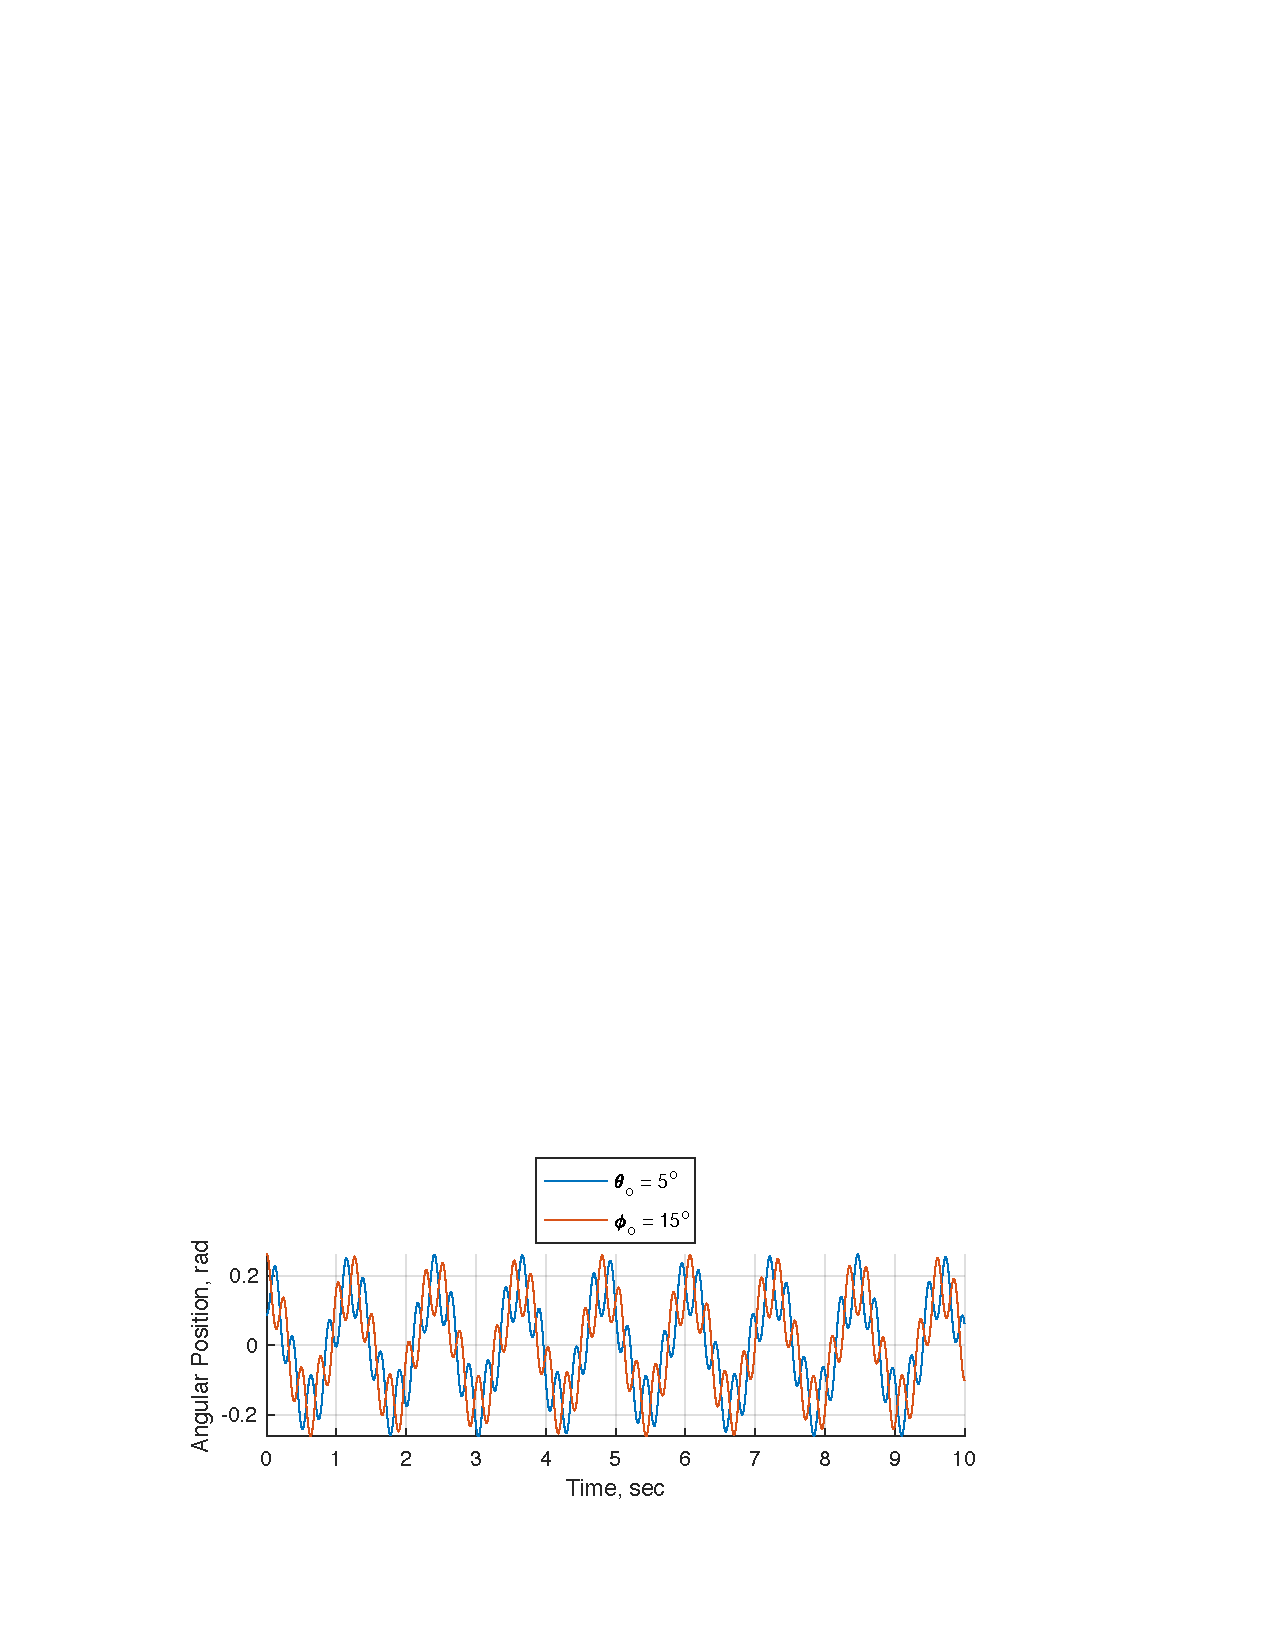
\includegraphics[center]{3}
  \caption{Angular Position vs. Time ($\theta_o:~5^\circ,~\phi_o:~15^\circ$)}
\end{figure}
% ---------------------------------------------------------------------------- %
\section{Does it Make Sense?}
% ---------------------------------------------------------------------------- %
\subsection{Units}

\subsection{Magnitude}

\section{Appendix} \label{appendix}

\subsection{Attributions}

\onehalfspacing
\begin{tabular}{ll}
Jeffrey Chen & \\
Thorne Wolfenbarger & \\
Trey Dufrene & \\
Joint Effort &
\end{tabular}
\singlespacing

\subsection{Analytical Solution}
\newpage
\subsection{Numerical Solution} \label{appendix:numerical}
\subsubsection{Non-Linearized}
\begin{lstlisting}[frame=lines,style=Matlab-editor]
clear;close all;clc

% Constants
c.m = 0.25; % kg
c.k = 25; % N/m
c.l = 0.5; % m
c.I = (1/3)*c.m*c.l^2; %kg.m^2
c.g = 9.81; % m/s^2

syms l g m k I theta phi thetadot thetaddot phidot phiddot...
    An At Cn Ct

% Cartesian locations of bar ends
b = l*[sin(theta);-cos(theta)];
d = l*[sin(phi)+1;-cos(phi)];
rbd = d - b;
rbdSquared = rbd.^2;
% Spring Length (mag)
ls = simplify(rbdSquared(1) + rbdSquared(2))^(1/2);
% Spring Direction (Left and Right)
ehatsL = (d - b) / ls;
ehatsR = (b - d) / ls;
% Normal / Tangential for Theta
ehatnT = [-sin(theta);cos(theta)];
ehattT = [cos(theta);sin(theta)];
% Normal / Tangential for Phi
ehatnP = [-sin(phi);cos(phi)];
ehattP = [cos(phi);sin(phi)];
% Spring Force (Left and Right)
FsL = k*(ls-l)*ehatsL;
FsR = k*(ls-l)*ehatsR;

% Spring force in normal direction (Theta)
Fs_nT = simplify(FsL(1)*ehatnT(1)+FsL(2)*ehatnT(2));
% Spring force in tangential direction (Theta)
Fs_tT = simplify(FsL(1)*ehattT(1)+FsL(2)*ehattT(2));

% Spring force in normal direction (Phi)
Fs_nP = simplify(FsR(1)*ehatnP(1)+FsR(2)*ehatnP(2));
% Spring force in tangential direction (Phi)
Fs_tP = simplify(FsR(1)*ehattP(1)+FsR(2)*ehattP(2));

% Sum of Normal Forces, left bar (Theta)
eqn(1) = m*(l/2)*thetadot^2 == Fs_nT + An - m*g*cos(theta);
% Sum of Tangential Forces, left bar (Theta)
eqn(2) = m*(l/2)*thetaddot == Fs_tT + At - m*g*sin(theta);
% Sum of Moments, left bar (Theta)
eqn(3) = -(l/2)*(m*g*sin(theta)) + (Fs_tT)*(l) == (1/3)*m*(l^2)*thetaddot;

% Sum of Normal Forces, right bar (Phi)
eqn(4) = m*(l/2)*phidot^2 == Fs_nP + Cn - m*g*cos(phi);
% Sum of Tangential Forces, right bar (Phi)
eqn(5) = m*(l/2)*phiddot == Fs_tP + Ct - m*g*sin(phi);
% Sum of Moments, right bar (Phi)
eqn(6) = -(l/2)*(m*g*sin(phi)) + (Fs_tP)*(l) == (1/3)*m*(l^2)*phiddot;

x = solve(eqn,[thetaddot,phiddot,An,At,Cn,Ct]);

syms theta(t) thetadot(t) phi(t) phidot(t)

thetaEOM = subs(x.thetaddot, {'theta', 'thetadot'}, {theta, thetadot});
phiEOM = subs(x.phiddot, {'phi', 'phidot'}, {phi, phidot});

eom = odeFunction([thetadot; thetaEOM; phidot; phiEOM],...
    [theta; thetadot; phi; phidot],m,k,l,I,g);

theta_o = [pi/12 -pi/12 pi/36];

for i = 1:3
    [T,S] = ode45(@(t,s)eom(t,s,c.m,c.k,c.l,c.I,c.g),linspace(0,10,1001),...
        [theta_o(i),0,pi/12,0]);
    figure
    hold on
    grid on
    xlabel('Time, sec')
    ylabel('Angular Position, rad')
    plot(T,S(:,1),'DisplayName', ['\theta_o = ' num2str(rad2deg(theta_o(i))) '^o'])
    plot(T,S(:,3),'DisplayName', '\phi_o = 15^o')
    legend('show')
end

% Checking EOM Units
u = symunit;
m = m*u.kg;
g = g*u.m/u.s^2;
l = l*u.m;
k = k*u.N/u.m;
An = An*u.N;
At = At*u.N;
Cn = Cn*u.N;
Ct = Ct*u.N;
theta = 'theta';
thetadot = 'thetadot'/u.s;
thetaddot = 'thetaddot'/u.s^2;
phi = 'phi';
phidot = 'phidot'/u.s;
phiddot = 'phiddot'/u.s^2;

eqn = subs(eqn);
unitCheck = checkUnits(eqn)
\end{lstlisting}
\color{gray} \begin{verbatim}
unitCheck =
  struct with fields:

    Consistent: [1 1 1 1 1 1]
    Compatible: [1 1 1 1 1 1]
\end{verbatim} \color{black}
\center
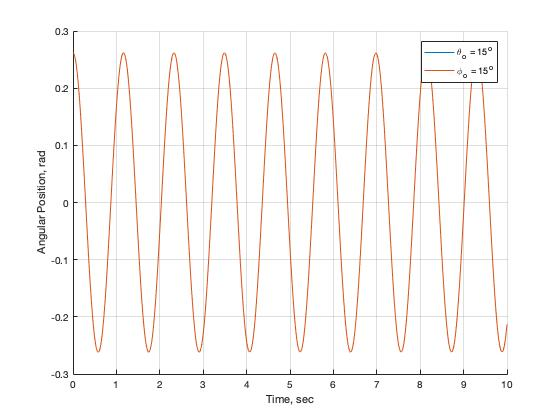
\includegraphics[center,width=4in]{rigid_01}

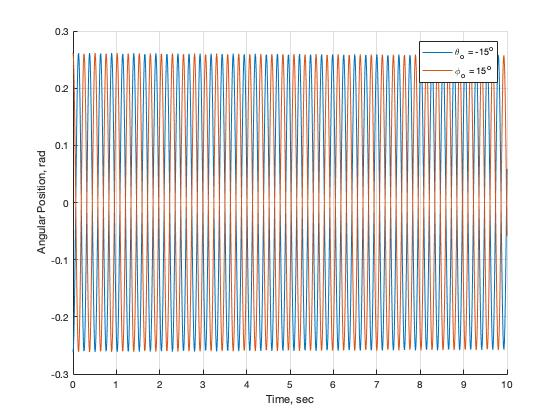
\includegraphics[center,width=4in]{rigid_02}

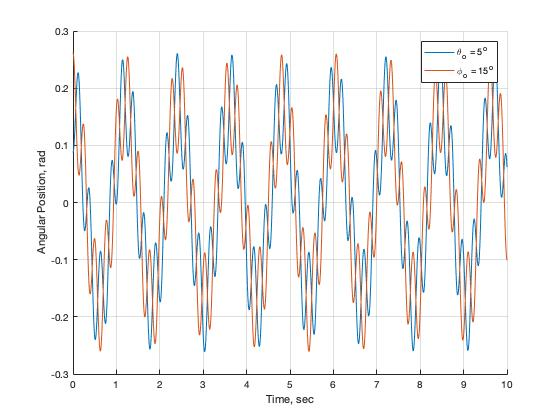
\includegraphics[center,width=4in]{rigid_03}


\end{flushleft}
\end{document}
